\section{Simulation study}
\label{sec:simulation}

The simulations assess five aspects of the method: recovery of the conditional
CDF, the transfer diagnostic, estimated borrowing under local misspecification,
risk scaling with local verified information, and simultaneous coverage. Within
each replication, all methods use the same observations, verification
indicators, folds, and threshold grid. The Supplement reports the complete
simulation designs, secondary learners, sensitivity analyses, and numerical
results.

\subsection{Design and estimands}

The common design draws
\[
X\sim U[-1,1],
\qquad
Y=\mu(X)+\sigma(X)\varepsilon,
\]
where \(\mu(x)=1.2x+0.6x^2\) and \(\sigma(x)=0.8+0.25x^2\). The baseline surrogate is \(S=Y+\tau_S\eta\), with independent standardized errors. Most experiments target \(x_0=0\) on a 101-point threshold grid corresponding to conditional probabilities from 0.02 to 0.98.

Mechanism and scarcity experiments use \(h=0.30\) and target \(F_{h,0}\); feasible point-estimation experiments use \(h=M^{-1/5}\) and target \(F_0\). Verification is random, bounded selective, or locally depleted near the target point, with probabilities calibrated to the stated mean reference fraction. Comparators are inverse-probability weighting, the \(X\)-based anchor, full surrogate borrowing, Adaptive, cross-validated shrinkage, and oracle variants.

The primary nuisance estimator is a location--scale model. Additional
experiments use misspecified parametric and nearest-neighbor regressions,
estimated verification probabilities, non-Gaussian and discrete outcomes, and
two-dimensional localization.

\begin{table}[H]
\centering
\small
\setlength{\tabcolsep}{3.5pt}
\caption{Finite-sample performance in the main simulation comparisons. ISE values are multiplied by $10^3$.}
\label{tab:simulation-headline}
\resizebox{\textwidth}{!}{%
\begin{tabular}{llrrrrrrr}
\toprule
Contrast & Setting & Anchor & Full & Adaptive & Gain (\%) & $E(\widehat\lambda_h)$ & NT Adaptive & NT Full \\
\midrule
Reference fraction & $p_M=0.05$ & 9.9 & 6.9 & 7.5 & 23.4 & 0.693 & 0.332 & 0.346 \\
 & $p_M=0.10$ & 4.8 & 3.5 & 3.6 & 24.0 & 0.784 & 0.339 & 0.360 \\
 & $p_M=0.20$ & 2.4 & 1.8 & 1.9 & 21.5 & 0.850 & 0.362 & 0.383 \\
Surrogate noise & $\tau_S=0.4$ & 4.9 & 2.3 & 2.5 & 48.5 & 0.835 & 0.203 & 0.222 \\
 & $\tau_S=0.8$ & 4.7 & 3.5 & 3.6 & 23.7 & 0.787 & 0.337 & 0.370 \\
 & $\tau_S=1.6$ & 4.7 & 4.3 & 4.4 & 7.6 & 0.683 & 0.429 & 0.443 \\
Sample size & $M=1{,}000$ & 8.2 & 6.3 & 6.6 & 19.1 & 0.713 & 0.379 & 0.391 \\
 & $M=4{,}000$ & 2.7 & 2.0 & 2.1 & 25.3 & 0.835 & 0.350 & 0.361 \\
Local reversal & N5 & 4.9 & 6.7 & 4.9 & -0.1 & 0.002 & 0.015 & 0.823 \\
\bottomrule
\end{tabular}%
}
\vspace{2pt}
\parbox{0.98\textwidth}{\footnotesize Gain is the percentage reduction in mean ISE from the anchor. Full uses borrowing weight one. NT is the frequency with which a method has larger ISE than the anchor in the same replication. N5 is the local-reversal setting.}
\end{table}


\begin{figure}[H]
\centering
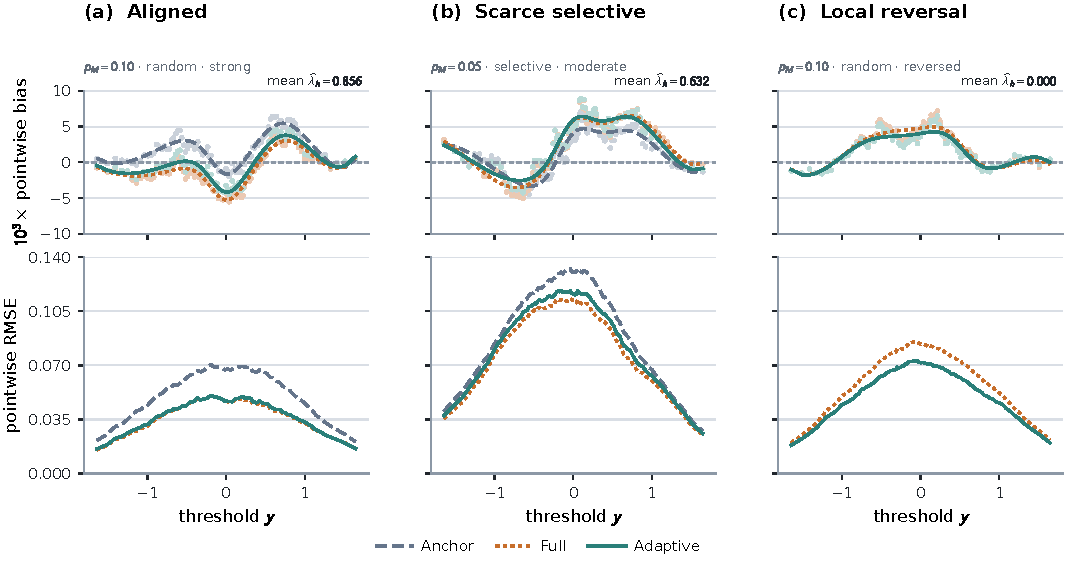
\includegraphics[width=\textwidth]{figures/figure1_distribution_recovery.pdf}
\caption{Pointwise recovery of the kernel-localized conditional CDF target $F_{h,0}(y\mid x_0)$ in three prespecified simulation settings. Columns show aligned borrowing, scarce selective verification, and local reversal. The upper row reports 1,000 times the Monte Carlo pointwise bias, defined as the mean rearranged estimate minus the target. Faint points are the unsmoothed biases; lines are inverse-Monte-Carlo-variance weighted cubic B-splines using the same five internal threshold knots for every curve. The horizontal reference is zero. The lower row reports pointwise RMSE on a common vertical scale. Each curve uses the same 500 Monte Carlo replications and 101-threshold grid. Full and Adaptive have lower RMSE than Anchor throughout the displayed grid in the aligned and scarce settings. Under local reversal, Adaptive tracks Anchor while Full has higher RMSE. No interval or confidence band is displayed.}
\label{fig:distribution-recovery}
\end{figure}

\subsection{Transfer direction and oracle-weight recovery}

% CLAIM_READY: SIM-H1
% CLAIM_READY: SIM-H2
% CLAIM_READY: SIM-H3
The oracle experiments vary the candidate correction while holding the
reference-outcome distribution, localization, and threshold grid fixed. M1 and
M2 favor full borrowing; M3 and M4 produce interior path-oracle weights; M5 and
M6 reverse the correction globally or near \(x_0\); and M7 and M8 introduce a
lower-tail failure or smooth model error. Each path is evaluated under random
and selective verification. The resulting 18 cells separate two questions:
whether \(2G_h-H_h\) predicts the risk direction of Full, and whether the
estimated coefficient recovers the minimum along the candidate path.

Oracle augmentation lowers mean ISE relative to the \(X\)-based anchor by
25.3--28.0\% in M1--M2. The conservative M2 correction improves on the anchor
without attaining the oracle-\(m\) risk, as predicted by the augmentation excess
covariance. Across all 18 cells, the sign of \(2G_h-H_h\) agrees with the paired
anchor-minus-Full ISE direction under both verification designs.

The clipped and raw M4 paths isolate the effect of path consistency. Clipping
changes the correction that enters the final estimator: the clipped
path has a positive transfer signal and a positive realized gain, whereas the
raw over-correction has a negative signal and increases ISE. Thus, the
diagnostic tracks the correction actually used by the estimator, including
transformations imposed before evaluation.

The estimated weight follows the same geometry. When
\(\lambda_h^{\mathrm{or}}=1\), its mean ranges from 0.852 to 0.998. The M3--M4
means remain close to their interior oracle values, and the lower-tail and
smooth-error paths retain substantial but incomplete borrowing. In the global
and local reversals, \(\lambda_h^{\mathrm{or}}=0\), the largest mean estimate is
below \(10^{-4}\), and Full increases risk. The mean absolute error between the
18 estimated and oracle cell means is 0.034.

\begin{figure}[H]
\centering
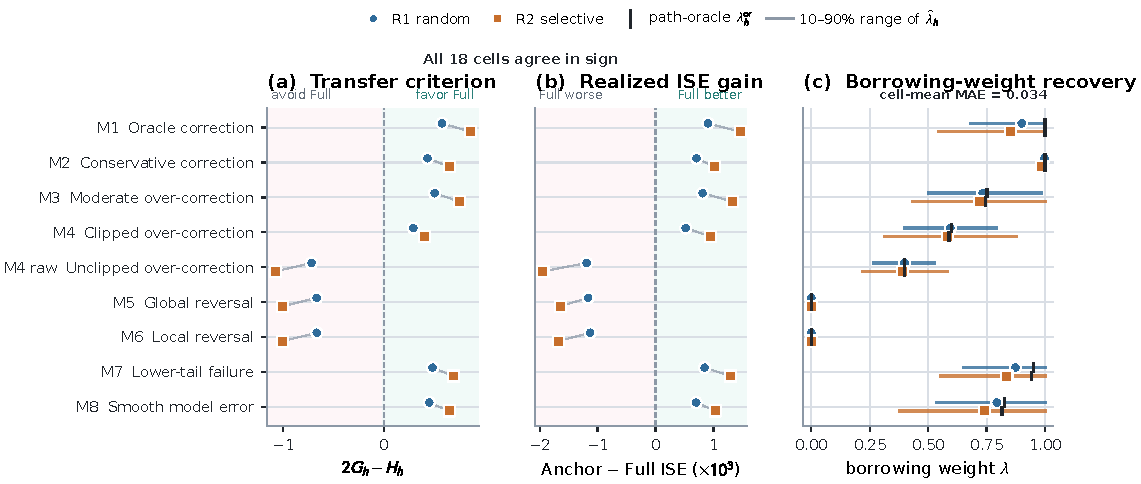
\includegraphics[width=\textwidth]{figures/figure2_transfer_geometry.pdf}
\caption{Transfer criterion, realized risk, and borrowing-weight recovery in
the oracle experiments. Rows index the eight candidate mechanisms, with the
clipped and raw M4 paths shown separately; circles denote R1 random
verification and squares R2 selective verification. Panels (a) and (b) report
the population criterion $2G_h-H_h$ and the paired Monte Carlo contrast
$10^3\{\operatorname{ISE}(\mathrm{Anchor})-
\operatorname{ISE}(\mathrm{Full})\}$. Positive values favor Full in both
panels, and the signs agree in all 18 cells. Thin gray segments
join the two verification designs for the same candidate path. Panel (c)
shows the path-oracle weight (black tick), mean selected weight (colored
marker), and empirical 10th--90th percentiles (colored segment; 2,000
replications for the primary paths and 1,000 for the raw M4 path); the mean
absolute error across the 18 cell means is 0.034.}
\label{fig:transfer-geometry}
\end{figure}

\subsection{Adaptive borrowing under misspecification}

% CLAIM_READY: SIM-H4
% CLAIM_READY: SIM-H5
The feasible experiments replace the oracle paths by regressions fitted within
the three-way rotation. Along the reference-fraction sequence in
Table~\ref{tab:simulation-headline}, Adaptive reduces mean final-CDF ISE by
21.5--24.0\%; absolute risk falls with \(p_M\), while the mean weight rises from
0.693 to 0.850. Surrogate quality has a larger effect on the value of
borrowing: the gain falls from 48.5\% at \(\tau_S=0.4\) to 7.6\% at
\(\tau_S=1.6\), accompanied by a decrease in the mean weight from 0.835 to
0.683. Increasing \(M\) from 1,000 to 4,000 raises the gain from 19.1\% to
25.3\% and the mean weight from 0.713 to 0.835.

Full has the lowest mean ISE in these aligned cells because Adaptive estimates
its coefficient on a separate selection fold. That gap contracts with local
information. The Adaptive-minus-fitted-path-oracle ISE difference decreases
from \(7.17\times10^{-4}\) to \(3.69\times10^{-5}\) as \(p_M\) rises from 0.05
to 0.20, and from \(4.29\times10^{-4}\) to \(4.24\times10^{-5}\) as \(M\)
rises from 1,000 to 4,000. Adaptive has no higher negative-transfer frequency
than Full in all 15 primary learner-by-quality cells and in seven of eight
nuisance-stress cells.

The misspecified regression learners preserve the main risk pattern. At
moderate surrogate noise, Adaptive gains are 23.7\%, 25.3\%, and 22.4\%
for the primary, misspecified parametric, and nearest-neighbor candidates. Over
the strong-to-weak surrogate sequence, the corresponding gain ranges are
48.5--7.6\%, 49.8--11.0\%, and 37.0--8.0\%. The three learners differ in how
much of the available surrogate information they recover, but all preserve the
declining gain as the surrogate becomes noisier.

In the local-reversal setting N5, Adaptive estimates a mean weight of 0.0017
and has a negative-transfer frequency of 1.5\%, compared with 82.3\% for Full.
A small number of loss realizations leave its mean ISE 0.066\% above the
anchor.

The vanishing-path experiment addresses the weak-curvature case in
Theorem~\ref{thm:oracle-equivalence}. For path scales
\(s\in\{1,0.5,0.25,0.125,0\}\), relative curvature follows \(s^2\), the
effective correction \(sE(\widehat\lambda_h)\) decreases from 0.899 to zero,
and the Adaptive-minus-path-oracle ISE gap decreases from
\(6.01\times10^{-5}\) to zero. Coefficient identification weakens with the
path, while the correction entering the CDF disappears at the same time.

\subsection{Verification scarcity and simultaneous bands}

% CLAIM_READY: SIM-H6
For local-information rate indices \(Mp_Mh\ge30\), scaled ISE ranges from
0.319 to 0.358 for the anchor and from 0.241 to 0.286 for Adaptive. Selective
verification changes the covariance constant even at the same nominal
reference fraction, so local precision depends on verification allocation as
well as the reference count.

The rescaled risks are stable over combinations of \(M\) and \(p_M\) that
produce the same rate index. Above 30, their coefficients of variation are
0.032 for the anchor and 0.052 for Adaptive. At indices 7.5 and 15, the
remaining variation is larger, consistent with the small local reference
samples. The ordering of the two methods persists throughout the grid, while
the separation between random and selective verification remains after rate
normalization because inverse-probability weighting changes the limiting
covariance constant.

\begin{figure}[H]
\centering
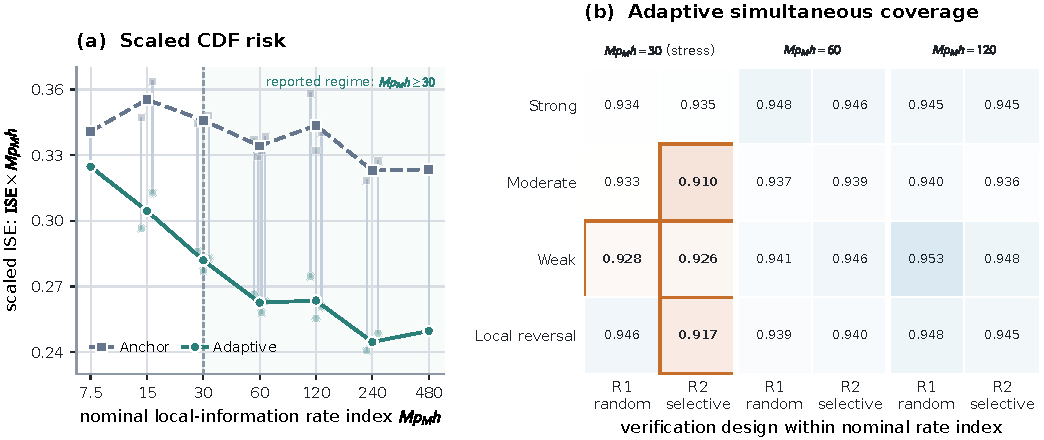
\includegraphics[width=\textwidth]{figures/figure3_scarcity_inference.pdf}
\caption{Risk scaling and raw-process simultaneous inference for the
kernel-localized target $F_{h,0}$ under scarce reference outcomes. In panel
(a), each thin vertical segment joins the Anchor and Adaptive mean scaled ISE
from the same scarcity setting; the large points and lines are
unweighted cell means at each nominal rate index. Each scenario uses 1,000
replications, and the shaded region marks the reported scaling regime
$Mp_Mh\geq30$; the spread across scenarios is not an uncertainty interval.
Panel (b) reports Adaptive empirical coverage of the 95\% raw-process
simultaneous band over 1,000 replications and 4999 multiplier draws per
replication. Cell color is centered at 0.95, and outlined bold cells are below
0.93; binomial Monte Carlo standard errors range from 0.0067 to 0.0090.
Supplementary Table S4 gives Anchor coverage and integrated widths, and Table
S5 gives the corresponding local-support diagnostic.}
\label{fig:scarcity-inference}
\end{figure}

% CLAIM_READY: SIM-H7
The band grid uses nominal rate indices \(Mp_Mh=30,60,120\); the first is a
deliberately low-information stress regime. In its selective-verification
cells, Adaptive and the anchor both under-cover. The minimum Adaptive estimate,
0.910, has Monte Carlo standard error 0.0090. The minimum role-fold verified
support averages about five in these cells. Pooled over the band grid, Adaptive
coverage increases from 0.875 at counts 0--3 to 0.911 at counts 4--5, 0.943 at
counts 6--9, and 0.945 when the count is at least 10. The minimum count across
the fitting, selection, and evaluation roles is therefore more informative for
finite-sample calibration than the global reference fraction alone.

Across all 24 cells, Adaptive coverage ranges from 0.910 to 0.953. Under
selective verification, mean coverage increases from 0.922 at \(p_M=0.05\) to
0.944 at \(p_M=0.20\). Strong aligned surrogates reduce integrated width to
0.760--0.981 of the anchor width; local reversal produces ratios of
1.000--1.003 because the fitted path contributes almost no correction. A
prespecified sensitivity increased endpoint rearrangement in seven cells and
improved several low-information coverages without removing the common
shortfall. Pointwise studentization reduced coverage to 0.358--0.633, so the
raw-process band remained the primary procedure.

\subsection{Robustness across outcomes and nuisance fits}

% CLAIM_READY: SIM-H8
The non-Gaussian experiments replace the normal error while retaining the same
conditional mean, scale, and surrogate construction. Adaptive gains are
15.6\%, 17.8\%, and 24.7\% under standardized \(t_3\), standardized
\(\chi^2_3\), and Gaussian-mixture errors, compared with 22.0\% under normal
errors. The method continues to borrow under heavy tails and skewness, but the
gain changes with the thresholdwise regression difficulty.

For a ten-level ordered outcome, category-scale oracle truth gives a 22.5\%
Adaptive gain and a 25.9\% Full gain. The target and risk are evaluated on the
support of the discrete outcome, matching the finite-grid process result.

The two-dimensional experiments use \(X=(X_1,X_2)\), a product Epanechnikov
kernel, and \(h=M^{-1/6}\). Across \(M\in\{2{,}000,5{,}000\}\) and
\(p_M\in\{0.10,0.20\}\), Adaptive gains range from 20.9\% to 24.4\%. The
larger neighborhoods required in two dimensions follow the effective
information scale \(Mp_Mh^d\).

Eight exploratory configurations estimate the verification probability on the
fitting fold. Adaptive gains range from 22.9\% to 45.4\%, with mean weights
from 0.408 to 0.600. The evaluated designs retain a risk benefit after the
verification model is estimated. Process inference with a
learned verification model uses the local product-rate and drift conditions
stated in the Supplement.
